% Copyright 2004 by Till Tantau <tantau@users.sourceforge.net>.
%
% In principle, this file can be redistributed and/or modified under
% the terms of the GNU Public License, version 2.

% However, this file is supposed to be a template to be modified
% for your own needs. For this reason, if you use this file as a
% template and not specifically distribute it as part of a another
% package/program, I grant the extra permission to freely copy and
% modify this file as you see fit and even to delete this copyright
% notice. 

\documentclass{beamer}

% There are many different themes available for Beamer. A comprehensive
% list with examples is given here:
% http://deic.uab.es/~iblanes/beamer_gallery/index_by_theme.html
% You can uncomment the themes below if you would like to use a different
% one:
%\usetheme{AnnArbor}
%\usetheme{Antibes}
%\usetheme{Bergen}
%\usetheme{Berkeley}
%\usetheme{Berlin}
%\usetheme{Boadilla}
%\usetheme{boxes}
%\usetheme{CambridgeUS}
%\usetheme{Copenhagen}
%\usetheme{Darmstadt}
%\usetheme{default}
%\usetheme{Frankfurt}
%\usetheme{Goettingen}
%\usetheme{Hannover}
%\usetheme{Ilmenau}
%\usetheme{JuanLesPins}
%\usetheme{Luebeck}
\usetheme{Madrid}
%\usetheme{Malmoe}
%\usetheme{Marburg}
%\usetheme{Montpellier}
%\usetheme{PaloAlto}
%\usetheme{Pittsburgh}
%\usetheme{Rochester}
%\usetheme{Singapore}
%\usetheme{Szeged}
%\usetheme{Warsaw}

\usecolortheme{beaver}
\usepackage{listings}
\usepackage{minted}
\usepackage{tikz}
\usetikzlibrary{shapes.geometric, arrows}
\usepackage{svg}
\usepackage{graphicx}
\graphicspath{{images/}}

\setbeamertemplate{itemize/enumerate body begin}{\LARGE}
\setbeamertemplate{itemize/enumerate subbody begin}{\large}

\newcommand{\shellcmd}[1]{\\\indent\indent\texttt{\footnotesize\# #1}\\}

\title{MIT-IIT Robotics Program}

% A subtitle is optional and this may be deleted
\subtitle{Logic Flow -- Booleans, Logical \& Relational Operators, Conditionals, While Loops}

\author{Amartya Shankha Biswas}%\inst{1}}
% - Give the names in the same order as the appear in the paper.
% - Use the \inst{?} command only if the authors have different
%   affiliation.

% - Use the \inst command only if there are several affiliations.
% - Keep it simple, no one is interested in your street address.

\date{\today}
% - Either use conference name or its abbreviation.
% - Not really informative to the audience, more for people (including
%   yourself) who are reading the slides online

% Delete this, if you do not want the table of contents to pop up at
% the beginning of each subsection:
\AtBeginSubsection[]
{
  \begin{frame}<beamer>{Outline}
    \tableofcontents[currentsection,currentsubsection]
  \end{frame}
}

% Let's get started
\begin{document}

\begin{frame}
  \titlepage
\end{frame}

\begin{frame}{Outline}
  \tableofcontents`
  % You might wish to add the option [pausesections]
\end{frame}

% Section and subsections will appear in the presentation overview
% and table of contents.

\section{Indian Computing Olympiad}

\begin{frame}[fragile]{IARCS}{}
\begin{figure}
    \begin{center}
        
\includegraphics[width=\linewidth]{images/iarcs.png}
    \end{center}
\end{figure}
\end{frame}

\begin{frame}[fragile]{Levels}{}
\begin{figure}
    \begin{center}
        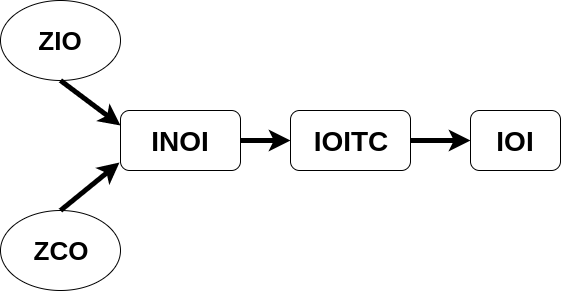
\includegraphics[width=\linewidth]{images/ico.png}
    \end{center}
\end{figure}
\end{frame}


\section{Processing Graphics}

\subsection{Getting Started}
\begin{frame}[fragile]{Installing}{}
\end{frame}

\begin{frame}[fragile]{}{}
    \Large
    \begin{minted}{c++}
        fill(0); //Set fill color
        ellipse(a, b, c, d);
    \end{minted}
    \pause
    \begin{minted}{text}
        a  float: x-coordinate of ellipse
        b  float: y-coordinate of ellipse
        c  float: width of the ellipse
        d  float: height of the ellipse
    \end{minted}
\end{frame}

\begin{frame}[fragile]{Window Size}{}
    \Large
    \begin{minted}{c++}
    int displayWidth = 800;
    int displayHeight = 400;
    \end{minted}
    \pause
    \begin{minted}{c++}
    size(displayWidth, displayHeight);
    \end{minted}
    \pause
    \begin{minted}{c++}
    // The wrong way to specify
    // the middle of the screen
    ellipse(400, 200, 50, 50);
    \end{minted}
    \pause
    \begin{minted}{c++}
    // Always the middle
    // no matter how size() changes
    ellipse(width/2, height/2, 50, 50);
    \end{minted}
\end{frame}

\subsection{Logic Flow}
\begin{frame}[fragile]{Flow}{}
\begin{figure}
    \begin{center}
        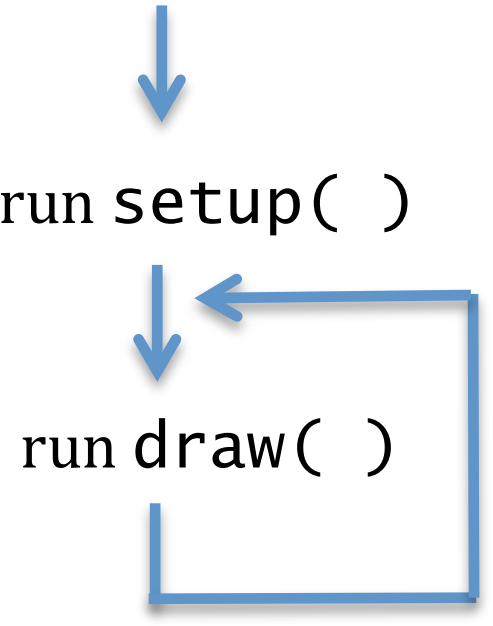
\includegraphics[width=0.8\linewidth]{images/setup_draw.png}
    \end{center}
\end{figure}
\end{frame}

\begin{frame}[fragile]{Setup and Loop}{}
    \begin{minted}{c++}
int displayWidth = 800;
int displayHeight = 400;
    \end{minted}
    \pause
    \begin{minted}{c++}
void setup (){
    size(displayWidth, displayHeight);
}
    \end{minted}
    \pause
    \begin{minted}{c++}
void draw (){
    background(255);
    fill(0);
    ellipse(width/2, height/2, 50, 50);
}
    \end{minted}
\end{frame}



\section{Functions}

\subsection{Definition}
\begin{frame}[fragile]{What is a Function ?}{}
    \LARGE
    \begin{block}{}
        A reusable block of code that performs a task.
    \end{block}
    \pause
    \begin{itemize}
        \item written by you and used by someone else
        \item written by someone else and used by you
    \end{itemize}
    \pause
    \begin{block}{}
        Don't need to know what the code looks like !
    \end{block}
\end{frame}

\begin{frame}[fragile]{What is a Function ?}{}
\begin{figure}
    \begin{center}
        
\includegraphics[width=0.7\linewidth]{images/bb.png}
    \end{center}
\end{figure}
\end{frame}


\subsection{Examples}

\begin{frame}[fragile]{You have already seen some functions.}{}
    \begin{itemize}
        \item main()
        \item sqrt(81)
        \item setup()
        \item draw()
        \item ellipse(50. 60, 10, 10)
        \item fill(255)
    \end{itemize}
\end{frame}

\begin{frame}[fragile]{The ellipse function.}{}
    \LARGE
    \begin{block}{Inputs to the ellipse() function}
        Coordinates of center. Size of ellipse.
    \end{block}
        \pause
    \begin{block}{What does the ellipse() function do ?}
        \pause
        Draws an ellipse on the screen, with specified parameters.
    \end{block}
        \pause
    \begin{block}{How ?}
        \pause
        Who cares ? . . .
    \end{block}
\end{frame}

\begin{frame}[fragile]{What do all functions have in common ?}{}
    \begin{itemize}
        \item main()
        \item sqrt(81)
        \item draw()
        \item ellipse(50, 60, 10, 10)
        \item fill(255)
    \end{itemize}
    \vfill
    \Huge Parentheses ()
\end{frame}


\subsection{Defining Functions}
\begin{frame}[fragile]{The structure of a Function}{}
\begin{figure}
    \begin{center}
        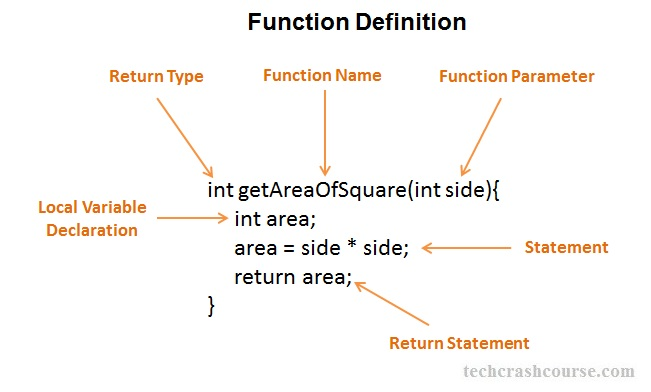
\includegraphics[width=0.8\linewidth]{images/func_label.jpg}
    \end{center}
\end{figure}
\end{frame}

\begin{frame}[fragile]{Control Flow}{}
\begin{figure}
    \begin{center}
        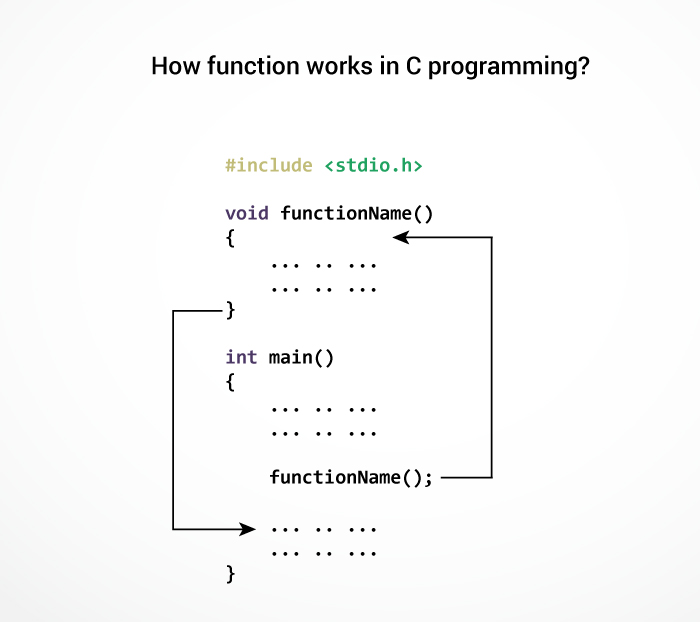
\includegraphics[width=0.8\linewidth]{images/func_flow.jpg}
    \end{center}
\end{figure}
\end{frame}

\begin{frame}[fragile]{Input to a Function}{}
\begin{figure}
    \begin{center}
        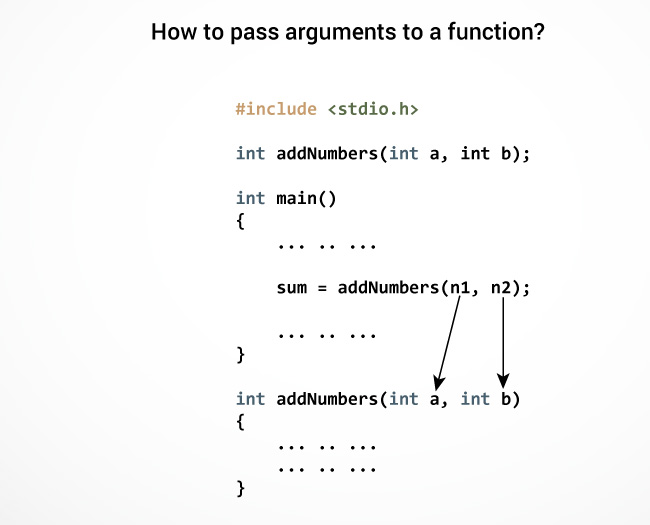
\includegraphics[width=0.8\linewidth]{images/func_args.jpg}
    \end{center}
\end{figure}
\end{frame}

\begin{frame}[fragile]{Return Value (output) of a Function}{}
\begin{figure}
    \begin{center}
        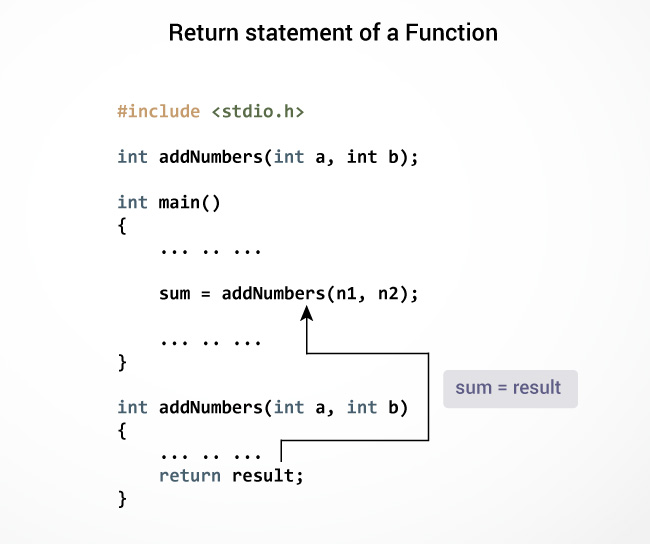
\includegraphics[width=0.8\linewidth]{images/func_return.jpg}
    \end{center}
\end{figure}
\end{frame}

\begin{frame}[fragile]{Exercise}{}
    \large
    \begin{block}{}
    Write a function drawTarget(), that takes $x$ and $y$ coordinate as input,
    and displays a target (concentric black and white circles) in that location.
    \end{block}
    \begin{block}{}
    Modify this function to take one integer N as input, and draw a target with N circles.
    This means that drawTarget(5) should display a target with 5 concentric circles.
    \end{block}
    \begin{block}{}
        Use this code to test.
        \begin{minted}{c++}
    void draw () {
        if (mousePressed) {
            drawTarget(mouseX, mouseY);
            delay(200);
        }
    }
        \end{minted}
    \end{block}
\end{frame}


\section{More on Processing}

\subsection{Primitives}
\begin{frame}[fragile]{Window Size}{}
    \Large
    \begin{minted}{c++}
        int width = 800;
        int height = 400;
    \end{minted}
    \pause
    \begin{minted}{c++}
        size(width, height);
    \end{minted}
    \pause
    \begin{minted}{c++}
        // The wrong way to specify
        // the middle of the screen
        ellipse(400, 200, 50, 50);
    \end{minted}
    \pause
    \begin{minted}{c++}
        // Always the middle
        // no matter how size() changes
        ellipse(width/2, height/2, 50, 50);
    \end{minted}
\end{frame}

\begin{frame}[fragile]{Rectangle}{}
    \Large
    \begin{minted}{c++}
        rect(a, b, c, d);
        rect(a, b, c, d, r);
        rect(a, b, c, d, tl, tr, br, bl);
    \end{minted}
    \pause
    \begin{minted}{text}
    a   float: x-coordinate of rectangle
    b   float: y-coordinate of rectangle
    c   float: width of the rectangle
    d   float: height of the rectangle
    \end{minted}
    \pause
    \begin{minted}{text}
    r   float: radii for all four corners
    \end{minted}
    \pause
    \begin{minted}{text}
    tl  float: radius of top-left corner
    tr  float: radius of top-right corner
    br  float: radius of bottom-right corner
    bl  float: radius of bottom-left corner
    \end{minted}
\end{frame}

\begin{frame}[fragile]{rect() Examples}{}
\begin{figure}
    \begin{center}
        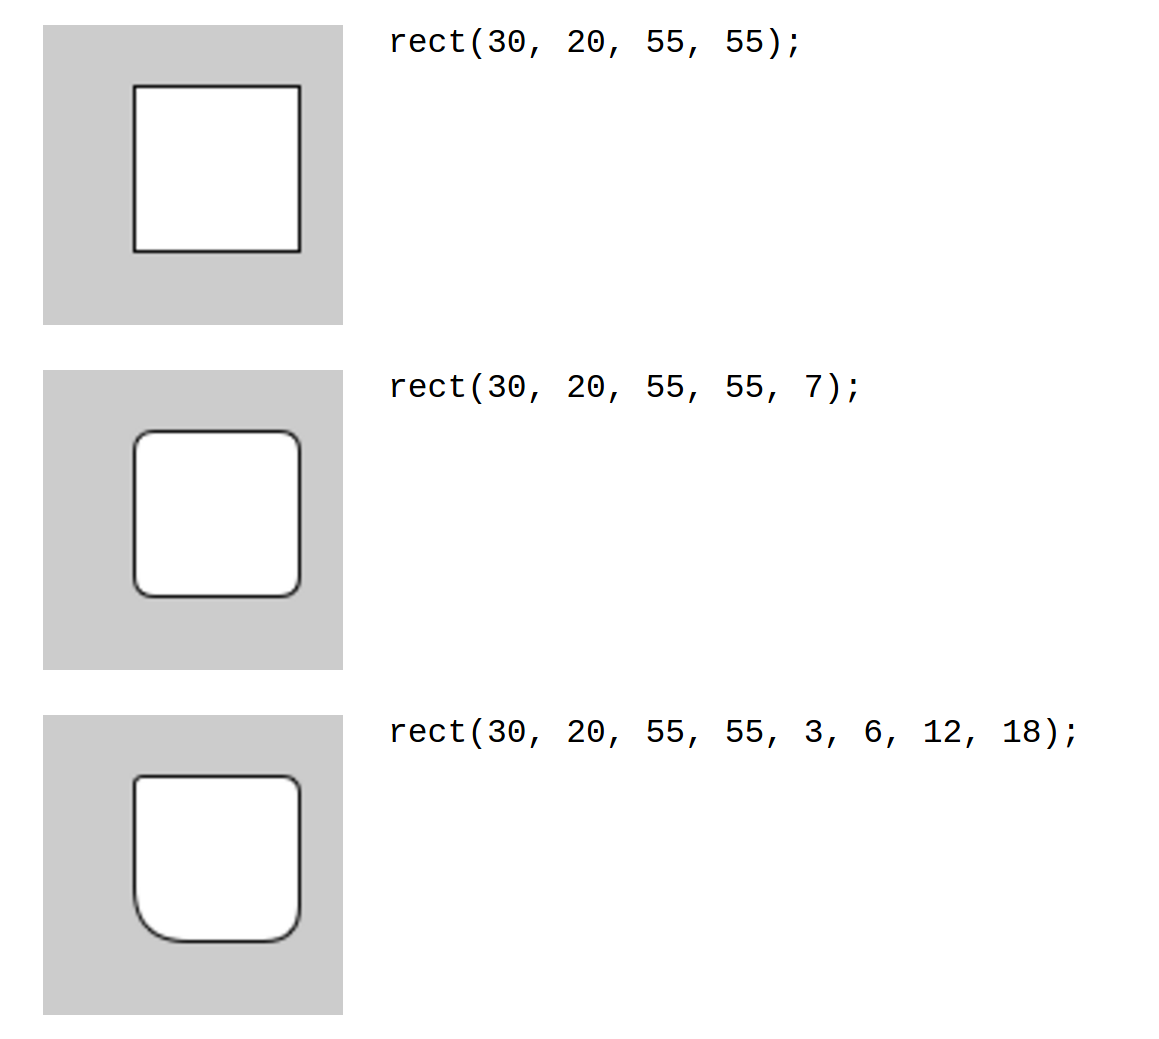
\includegraphics[width=.7\linewidth]{images/rect.png}
    \end{center}
\end{figure}
\end{frame}

\subsection{Coordinate System}
\begin{frame}[fragile]{Normal Coordinate System}{}
\begin{figure}
    \begin{center}
        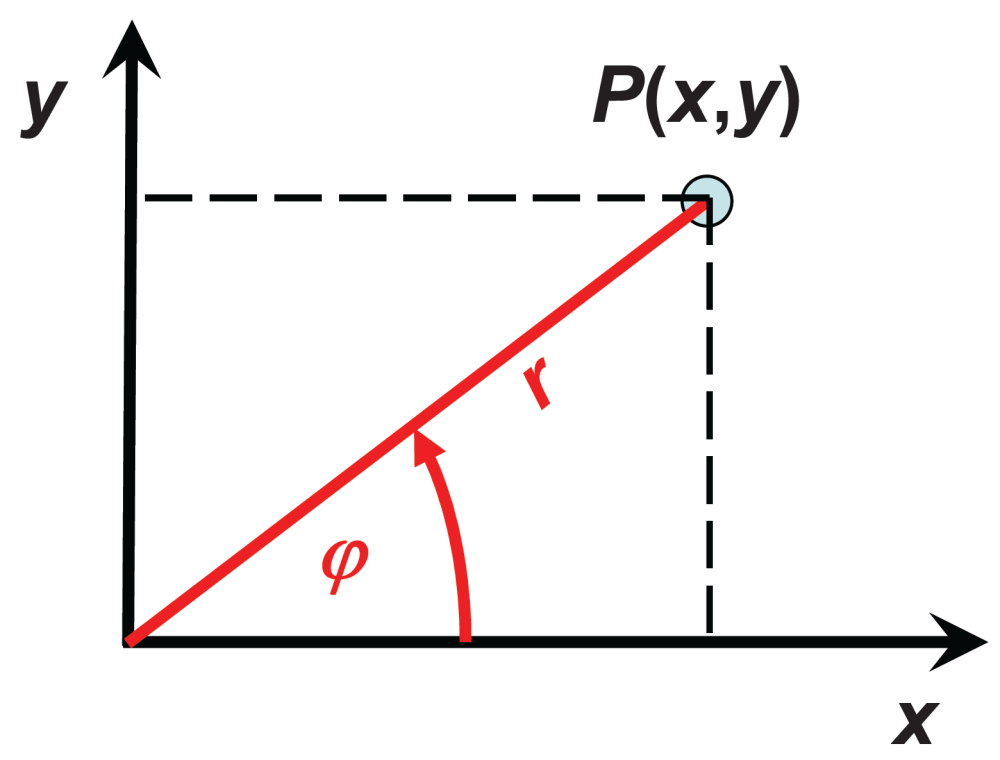
\includegraphics[width=.8\linewidth]{images/normal_coord.png}
    \end{center}
\end{figure}
\end{frame}

\begin{frame}[fragile]{Processing Coordinate System}{}
\begin{figure}
    \begin{center}
        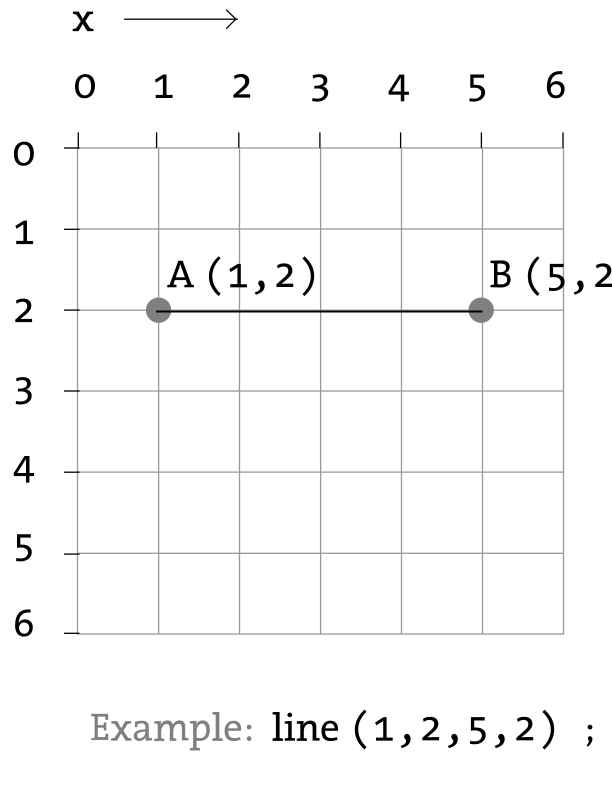
\includegraphics[width=.6\linewidth]{images/processing_coord.png}
    \end{center}
\end{figure}
\end{frame}

\begin{frame}[fragile]{Drawing a Rectangle}{}
\begin{figure}
    \begin{center}
        \def\svgwidth{\columnwidth}
        \input{images/rect_normal.pdf_tex}
    \end{center}
\end{figure}
\end{frame}

\begin{frame}[fragile]{CENTER Rectangle}{}
\begin{figure}
    \begin{center}
        \def\svgwidth{0.9\columnwidth}
        \input{images/rect_center.pdf_tex}
    \end{center}
\end{figure}
\end{frame}

\begin{frame}[fragile]{CORNERS Rectangle}{}
\begin{figure}
    \begin{center}
        \def\svgwidth{0.9\columnwidth}
        \input{images/rect_corners.pdf_tex}
    \end{center}
\end{figure}
\end{frame}


\subsection{Debugging}
\begin{frame}[fragile]{Print Statements}{}
    \begin{itemize}
    \item print() statement prints all items separated by spaces
    \begin{minted}{cpp}
    print(item1, item2, . . . );
    \end{minted}
    \pause
    \item println() is the same, but prints a new line at the end
    \begin{minted}{cpp}
    println(item1, item2, . . . );
    \end{minted}
    \end{itemize}
\end{frame}


\subsection{Interaction}
\begin{frame}[fragile]{Mouse Handling}{}
    \begin{itemize}
    \item Mouse position -- Global Variables
    \begin{minted}{cpp}
    mouseX, mouseY
    ellipse(mouseX, mouseY, 2*R, 2*R);
    \end{minted}
    \pause
    \item Detect Mouse Click
    \begin{minted}{cpp}
    if (mousePressed) {
       fill(255); // White
    } else {
        fill(0); // Black
    }
    \end{minted}
    \end{itemize}
\end{frame}

\begin{frame}[fragile]{Keyboard Handling}{}
    \Large
    \begin{minted}{cpp}
    char LEFT = 'a', RIGHT = 'd', UP = 'w';
    boolean left, right, up;
    \end{minted}
    \pause
    \begin{minted}{cpp}
    void keyPressed() {
        if (key == LEFT)       left = true;
        if (key == RIGHT)      right = true;
        if (key == UP)         up = true;
    }
    \end{minted}
    \pause
    \begin{minted}{cpp}
    void keyReleased() {
        if (key == LEFT)       left = false;
        if (key == RIGHT)      right = false;
        if (key == UP)         up = false;
    }
    \end{minted}
\end{frame}

\begin{frame}[fragile]{Keyboard Handling}{}
    \huge
    \begin{minted}{cpp}
    if (left) {
        // Move Left . . .
    }
    if (right) {
        // Move Right . . .
    }
    if (up) {
        // Move Up . . .
    }
    \end{minted}
\end{frame}

\subsection{Physics}
\begin{frame}[fragile]{Define Position and Velocity}{}
    \Large
    \begin{minted}{cpp}
    float ballX = width/2, ballY = height/2;
    float ballVx = 2, ballVy = 3;
    \end{minted}
    \pause
    \begin{minted}{cpp}
    void draw() {
        ellipse(ballX, ballY, 2*R, 2*R);
        updateBallPosition();
    }
    \end{minted}
    \pause
    \begin{minted}{cpp}
    void updateBallPosition() {
        ballX += ballVx;
        ballY += ballVy;
    }
    \end{minted}
\end{frame}

\begin{frame}[fragile]{Gravity}{}
    \Large
    \begin{minted}{cpp}
    float gravity = 1;
    \end{minted}
    \pause
    \begin{minted}{cpp}
    void draw() {
        ellipse(ballX, ballY, 2*R, 2*R);
        updateBallVelocity();
        updateBallPosition();
    }
    \end{minted}
    \pause
    \begin{minted}{cpp}
    void updateBallVelocity() {
        ballVy += gravity;
    }
    \end{minted}
\end{frame}


\subsection{Exercise}
\begin{frame}[fragile]{Forking}{}
    \begin{block}{}
        Go to https://github.com/amartyashankha/MIRP2017\_movement
    \end{block}
    \begin{block}{Click on Fork}
        \begin{figure}
            \begin{center}
                
\includegraphics[width=\linewidth]{images/git_fork.png}
            \end{center}
        \end{figure}
    \end{block}
    \begin{block}{The title should change}
        \begin{figure}
            \begin{center}
                
\includegraphics[width=\linewidth]{images/git_forked.png}
            \end{center}
        \end{figure}
    \end{block}
\end{frame}

\begin{frame}[fragile]{Cloning}{}
    \begin{block}{Clone the repo}
        \begin{figure}
            \begin{center}
                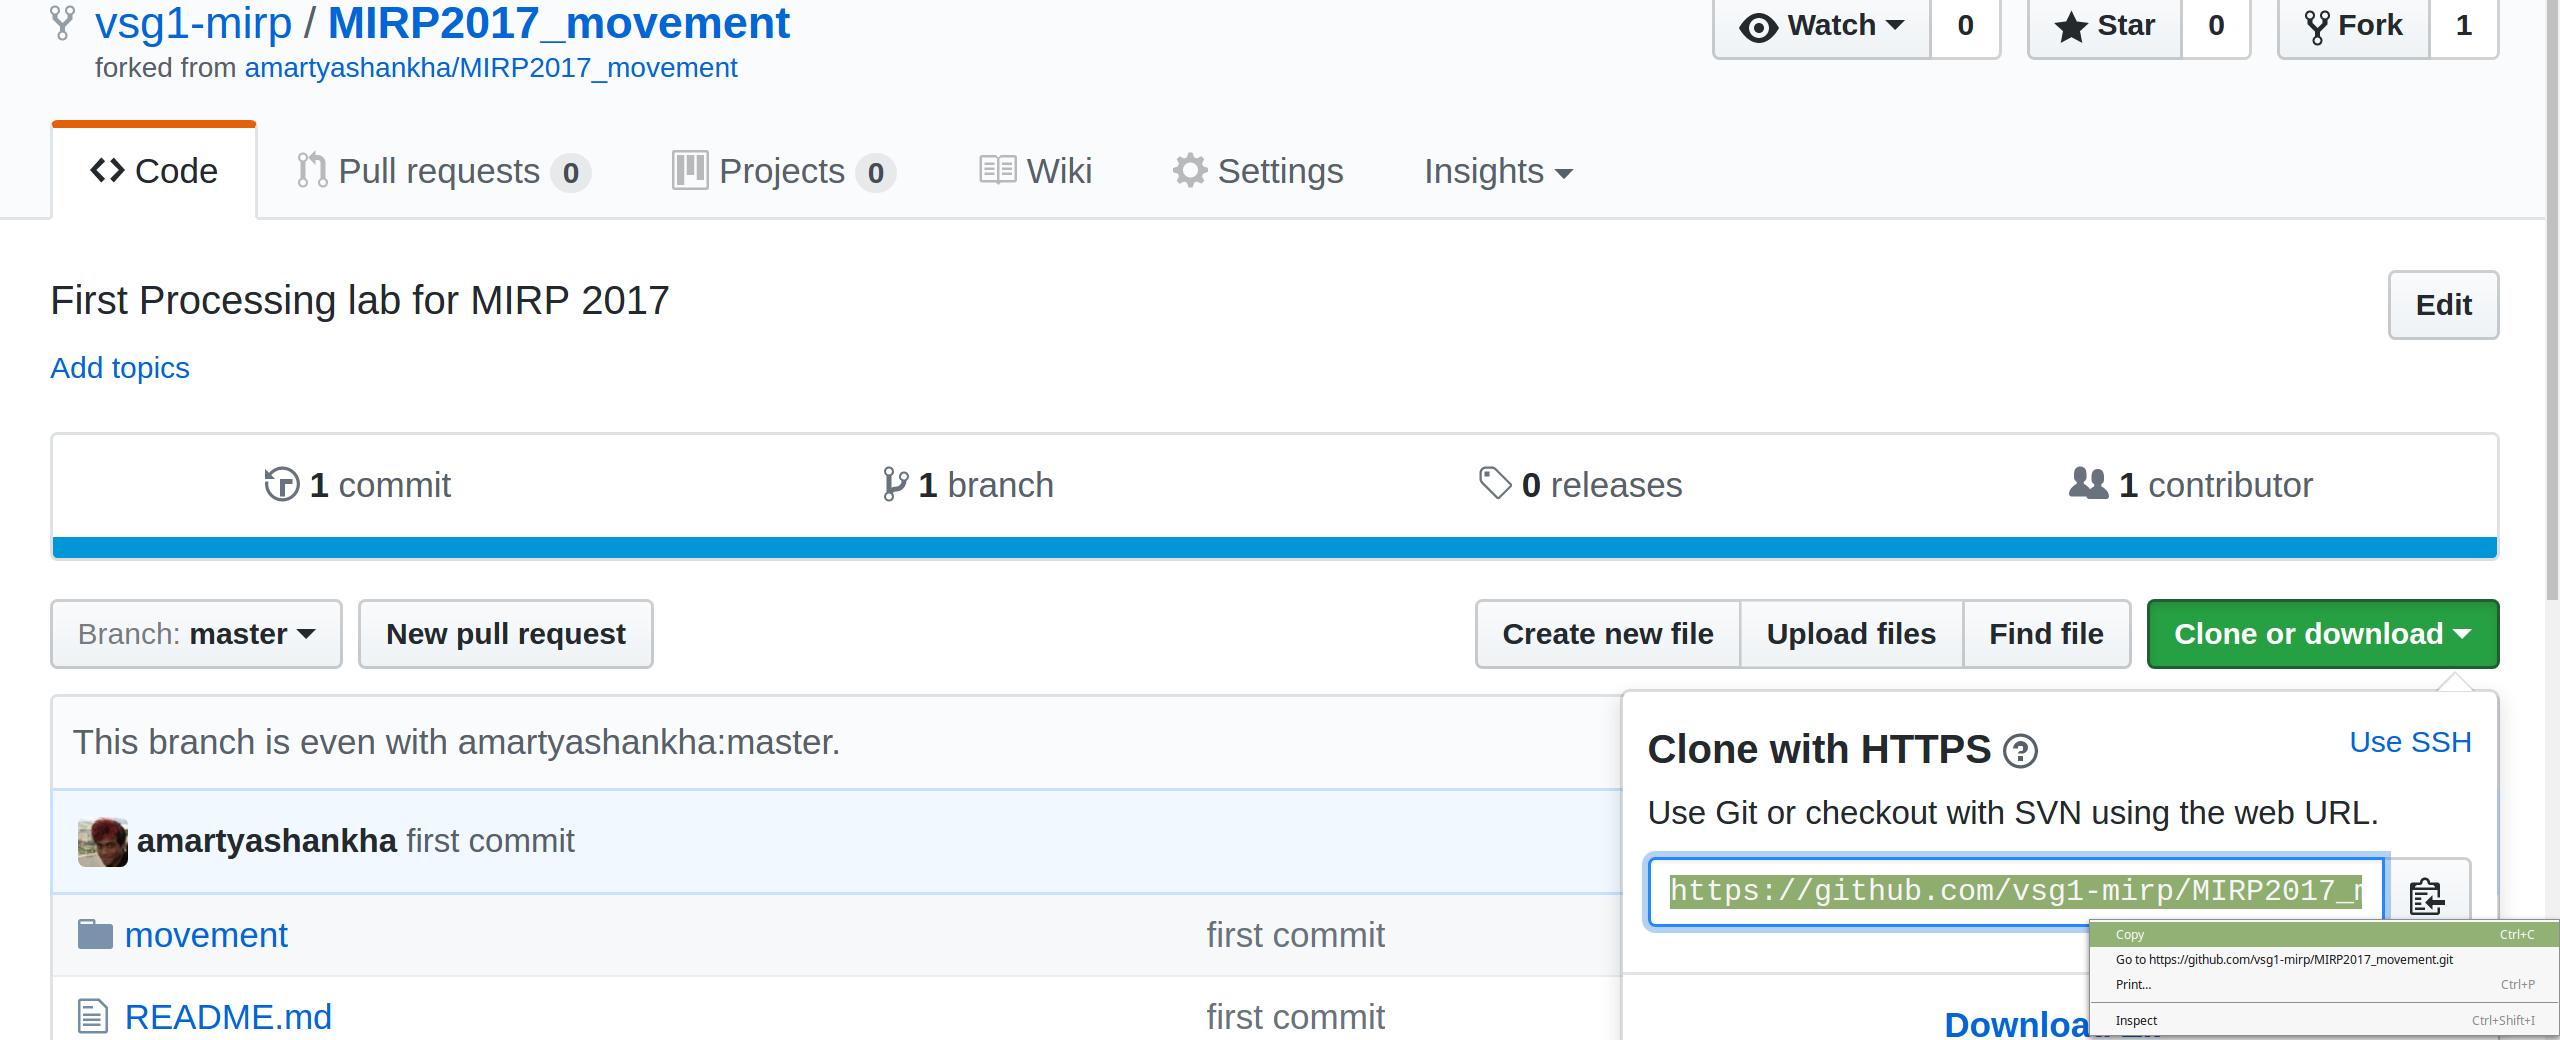
\includegraphics[width=0.8\linewidth]{images/git_clone.png}
            \end{center}
        \end{figure}
    \end{block}
    \begin{itemize}
        \item Open Processing
        \item File $\rightarrow$ Open
        \item Navigate to the files inside Movement 
    \end{itemize}
\end{frame}

\begin{frame}[fragile]{Exercise}{}
    \LARGE
    \begin{block}{}
    Resolve collisions with other walls.
    Move ball using WASD.
    \end{block}
    \begin{block}{}
    Move ball using WASD.
    \end{block}
\end{frame}



\end{document}


